
%%% Local Variables:
%%% TeX-master: t
%%% coding: utf-8
%%% mode: latex
%%% End:

\documentclass[notes]{beamer}
\usetheme{Boadilla}

\usepackage[utf8]{inputenc}
\usepackage[english]{babel}
\usepackage{framed}
\usepackage{graphicx}
\graphicspath{ {images/} }
\newcommand{\term}[1]{$\vcenter{\hbox{\includegraphics[scale=0.50]{#1.png}}}$}

\usepackage{xcolor}
\definecolor{light-gray}{gray}{0.90}
\makeatletter
\def\mathcolor#1#{\@mathcolor{#1}}
\def\@mathcolor#1#2#3{%
  \protect\leavevmode
  \begingroup
    \color#1{#2}#3%
  \endgroup
}
\makeatother


\usepackage{listings}
\lstdefinestyle{bnf}{
  mathescape,
  basicstyle=\footnotesize\ttfamily,
  breaklines=true
}

\lstdefinestyle{bnfsm}{
  mathescape,
  basicstyle=\scriptsize\ttfamily,
  breaklines=true
}

\usepackage{elm-highlighting}

\usepackage{changepage}
\usepackage{mathpartir}
\newcommand{\rulename}[1]{\textsc{\MakeLowercase{#1}}}
\newcommand{\derivRule}[3]{
  \inferrule*[Left=#1]{#3}{#2}
}
\newcommand{\derivTree}[3]{
  \inferrule*[Right=#1]{#3}{#2}
}


\usepackage{tikz-qtree}
\usepackage{tikz-qtree-compat}
\newcommand{\mybox}[1]{\setlength{\fboxsep}{0pt}\colorbox{orange!10}{#1}}

\title[Phometa]{\textbf{Phometa} --- a visualised proof assistant \\
       that builds a formal system and proves \\
       its theorems using derivation trees}
\author{Gun Pinyo}
\institute{Imperial College London}
\date{June 21, 2016}

\begin{document}

\frame{\titlepage}


\begin{frame}[fragile]
\frametitle{Derivation systems can reason many formal systems.}
$$
\derivRule{imply-elim, rightskip=3em}{\Gamma \vdash B}{\Gamma \vdash (A \rightarrow B) \\
  \Gamma \vdash A}
$$
\vspace{2em}
$$
\derivTree{and-intro,leftskip=6em}{p, p \rightarrow q \vdash p \wedge q}
  { \derivTree{ass}{p, p \rightarrow q \vdash p} { }
    \\
    \derivTree{imply-elim}{p, p \rightarrow q \vdash q}
    { \derivTree{ass}{p, p \rightarrow q \vdash p \rightarrow q} { }
      \\
      \derivTree{ass}{p, p \rightarrow q \vdash p} { }
    }
  }
$$
\end{frame}

\begin{frame}
\frametitle{Derivation systems can reason many formal systems.}
$$
\derivTree{mult-intro,leftskip=6em}{(((w \times x) + (w \times y)) \times z) =
                         ((w \times (x + y)) \times z)}
  { \derivTree{eq-symm}{((w \times x) + (w \times y)) =
                         (w \times (x + y))}
    { \derivTree{dist-left}{(w \times (x + y)) = ((w \times x) + (w \times y))} { }
    }
   \\ \\ \\
    { \derivTree{eq-refl}{z = z}{ }
    }
  }
$$
\vspace{3ex}
$$
\derivTree{arrow-elim,leftskip=6em}{y : A \vdash (\lambda x . x) y : A}
  { \derivTree{arrow-intro}{y : A \vdash \lambda x . x : A \rightarrow A}
    { \derivTree{assumption}{y : A, x : A \vdash x : A} { }
    }
  \\ \\ \\ \\
    \derivTree{assumption}{y : A \vdash y : A}{ }
  }
$$
\end{frame}

\begin{frame}
\frametitle{Problem of drawing a derivation tree.}
\begin{itemize}
  \item Its width grows exponentially to its height.
  \item One drawing mistake might need major correction of the entire tree.
  \item (Meta) is being rewritten by unification.
  \item Cannot systematically check that the tree has no errors.
\end{itemize}

\end{frame}

\begin{frame}
\frametitle{Screenshot of  ``Phometa'' in action}
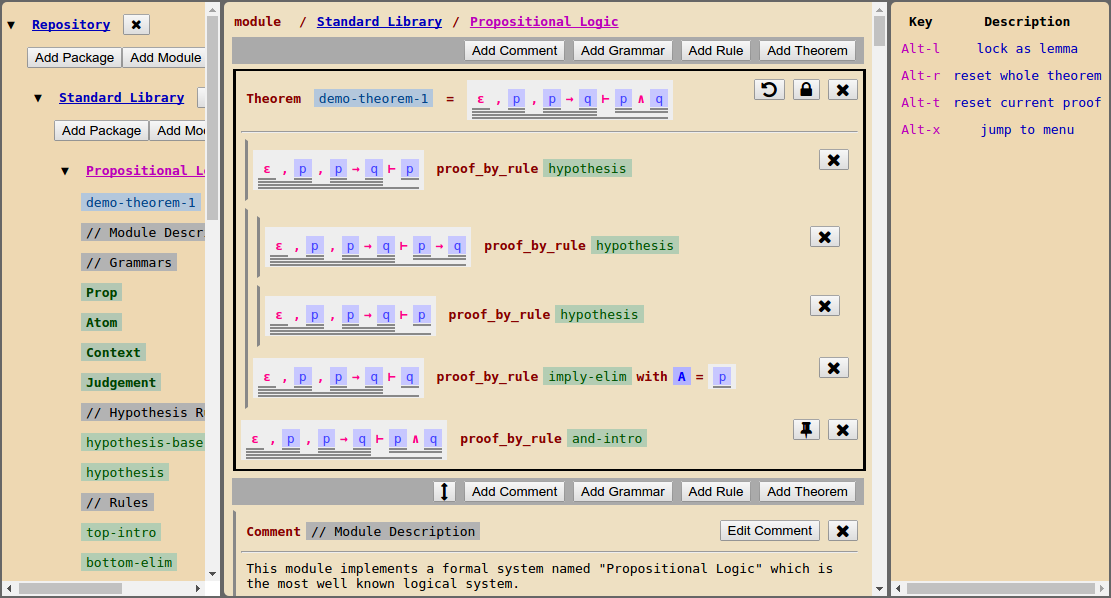
\includegraphics[width=\linewidth,height=\textheight,keepaspectratio]{demo-1}
\end{frame}

\begin{frame}[fragile]
\frametitle{Formal system ingredient - Grammar (Backus-Nour Form)}


\begin{minipage}{0.48\textwidth}
\begin{flushleft}
\begin{lstlisting}[style=bnfsm]
<Prop> ::= `$\top$' | `$\bot$' | <Atom>
   | `('<Prop> `$\wedge$' <Prop>`)'
   | `('<Prop> `$\vee$' <Prop>`)'
   | `( $\neg$' <Prop>`)'
   | `('<Prop> `$\rightarrow$' <Prop>`)'
   | `('<Prop> `$\leftrightarrow$' <Prop>`)'
   | meta-variable with regex
/[A-Z][a-zA-Z]*([1-9][0-9]*|'*)/
\end{lstlisting}
\vspace{2ex}
\Tree[.\mybox{\term{demo-term-1-1} is \term{demo-pgmr-prop}}
       [.\mybox{\term{demo-term-1-2} is \term{demo-pgmr-prop}}
         \mybox{\term{demo-term-1-3} is \term{demo-pgmr-prop}} ]
       [.\mybox{\term{demo-term-1-4} is \term{demo-pgmr-prop}}
         [.\mybox{\term{demo-term-1-5} is \term{demo-pgmr-prop}}
           \mybox{\term{demo-term-1-6} is \term{demo-pgmr-atom}} ]
         \mybox{\term{demo-term-1-7} is \term{demo-pgmr-prop}} ] ]
\end{flushleft}
\end{minipage}
~
\begin{minipage}{0.48\textwidth}
\begin{flushright}

\begin{lstlisting}[style=bnfsm]
<Atom> ::= literal with regex
/[a-z][a-zA-Z]*([1-9][0-9]*|'*)/
\end{lstlisting}
\vspace{2ex}
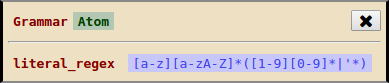
\includegraphics[width=\textwidth]{demo-gmr-atom} \\
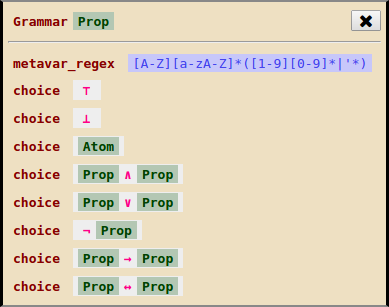
\includegraphics[width=\textwidth]{demo-gmr-prop}


\end{flushright}
\end{minipage}

\end{frame}



\begin{frame}[fragile]
\frametitle{Grammar (Backus-Nour Form)}


\begin{minipage}{0.58\textwidth}
\begin{flushleft}
\begin{lstlisting}[style=bnfsm]
<Context> ::= `$\epsilon$'
  | <Context> `,' <Prop>
  | meta-variables comply with regex
      /[$\Gamma\Delta$]([1-9][0-9]*|'*)/

<Judgement> ::= <Context> `$\vdash$' <Prop>
\end{lstlisting}
\end{flushleft}
\end{minipage}
~
\begin{minipage}{0.38\textwidth}
\begin{flushright}
\vspace{-2em}
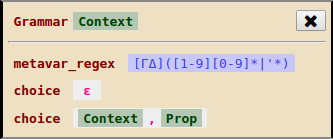
\includegraphics[width=\textwidth]{demo-gmr-context} \\
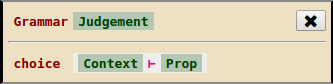
\includegraphics[width=\textwidth]{demo-gmr-judgement}
\end{flushright}
\end{minipage}
\Tree[.\mybox{\term{demo-term-2-1} is \term{demo-pgmr-judgement}}
       [.\mybox{\term{demo-term-2-2} is \term{demo-pgmr-context}}
         [.\mybox{\term{demo-term-2-3} is \term{demo-pgmr-context}}
           [.\mybox{\term{demo-term-2-4} is \term{demo-pgmr-context}}
           ]
           [.\mybox{\term{demo-term-2-p-} is \term{demo-pgmr-prop}}
             \mybox{\term{demo-term-2-p} is \term{demo-pgmr-atom}}
           ]
         ]
         [.\mybox{\term{demo-term-2-5} is \term{demo-pgmr-prop}}
           [.\mybox{\term{demo-term-2-p-} is \term{demo-pgmr-prop}}
             \mybox{\term{demo-term-2-p} is \term{demo-pgmr-atom}}
           ]
           [.\mybox{\term{demo-term-2-q-} is \term{demo-pgmr-prop}}
             \mybox{\term{demo-term-2-q} is \term{demo-pgmr-atom}}
           ]
         ]
       ]
       [.\mybox{\term{demo-term-2-6} is \term{demo-pgmr-prop}}
         [.\mybox{\term{demo-term-2-p-} is \term{demo-pgmr-prop}}
           \mybox{\term{demo-term-2-p} is \term{demo-pgmr-atom}}
         ]
         [.\mybox{\term{demo-term-2-q-} is \term{demo-pgmr-prop}}
           \mybox{\term{demo-term-2-q} is \term{demo-pgmr-atom}}
         ]
       ]
     ]
\end{frame}

\begin{frame}[fragile]
\frametitle{Formal system ingredient - Rule (Derivation Rule)}

$$
\derivRule{imply-elim, rightskip=3em}{\Gamma \vdash B}{\Gamma \vdash (A \rightarrow B) \\
  \Gamma \vdash A}
$$

\begin{minipage}{0.38\textwidth}
\begin{flushleft}
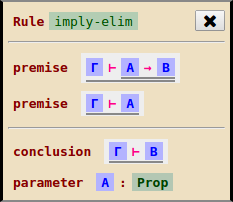
\includegraphics[width=\textwidth]{demo-rule-imply-elim}
\end{flushleft}
\end{minipage}
~
\begin{minipage}{0.58\textwidth}
\begin{flushright}
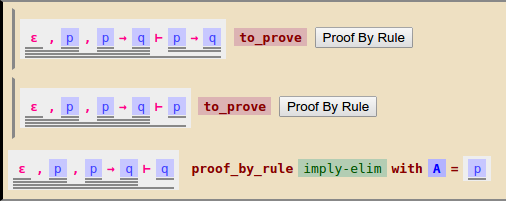
\includegraphics[width=\textwidth]{demo-sub-thm-1}
\vspace{-1em}
\begin{center}
\begin{tabular}{ l c c l }
 Pattern Matching & \term{demo-term-3-1} & $=$ & \term{demo-term-2-2} \\ [0.5em]
                  & \term{demo-term-3-2} & $=$ & \term{demo-term-2-q-} \\ [1em]
 Parameter(s)     & \term{demo-term-3-3} & $=$ & \term{demo-term-2-p-}
\end{tabular}
\end{center}
\end{flushright}
\end{minipage}

\end{frame}

\begin{frame}[fragile]
\frametitle{Formal system ingredient - Theorem (Derivation Tree)}
\begingroup
    \fontsize{10pt}{12pt}\selectfont
$$
\derivTree{and-intro,leftskip=6em}{p, p \rightarrow q \vdash p \wedge q}
  { \derivTree{ass}{p, p \rightarrow q \vdash p} { }
    \\
    \derivTree{imply-elim}{p, p \rightarrow q \vdash q}
    { \derivTree{ass}{p, p \rightarrow q \vdash p \rightarrow q} { }
      \\
      \derivTree{ass}{p, p \rightarrow q \vdash p} { }
    }
  }
$$
\endgroup
\begin{center}
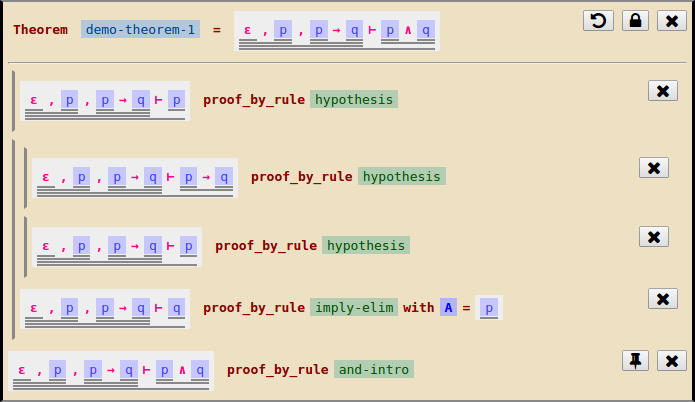
\includegraphics[width=0.8\linewidth,keepaspectratio]{demo-theorem-1}
\end{center}
\end{frame}

\begin{frame} [fragile]
\frametitle{Demonstration}

\begin{itemize}
\item Overview of Phometa's user interface.\\ [1em]

\item Prove that \term{demo-term-2-1} is a valid \term{demo-pgmr-judgement}.\\ [1em]

\item Extend Propositional Logic to support equivalence.\\ [1em]

\begin{adjustwidth}{4.5em}{0em}
\begin{lstlisting}[style=bnfsm]
<Equivalence> ::= <Prop> `$\equiv$' <Prop>
\end{lstlisting}
\end{adjustwidth}
\vspace{1em}
$$
\derivRule{equiv-intro, rightskip=3em}{A \equiv B}{A \vdash B \\
  B \vdash A}
$$

\item Prove that \term{demo-term-4-1} is a valid \term{demo-pgmr-equiv}.

\end{itemize}
\end{frame}

\begin{frame}
  \frametitle{Cascade Premise --- Hypothesis Rule}

\begin{center}
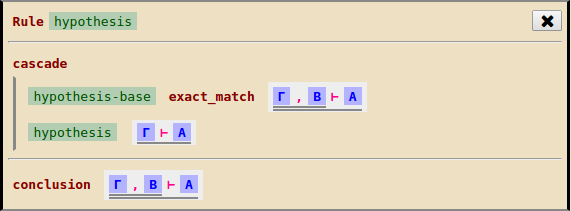
\includegraphics[width=0.8\linewidth,height=\textheight,keepaspectratio]{demo-rule-hypo}\\[1em]
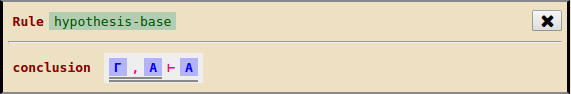
\includegraphics[width=0.8\linewidth,height=\textheight,keepaspectratio]{demo-rule-hypo-base}
\end{center}
\end{frame}


\begin{frame}
  \frametitle{Meta-Reduction --- Context Manipulation}

\begin{adjustwidth}{1em}{0em}
\begin{minipage}{0.50\textwidth}
\begin{flushleft}
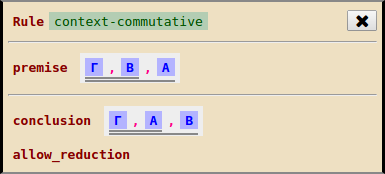
\includegraphics[width=\textwidth]{prop-context-comm}\\
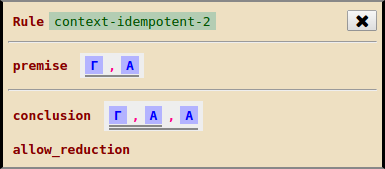
\includegraphics[width=\textwidth]{prop-context-idem-2}
\end{flushleft}
\end{minipage}
~
\begin{minipage}{0.40\textwidth}
\begin{flushright}
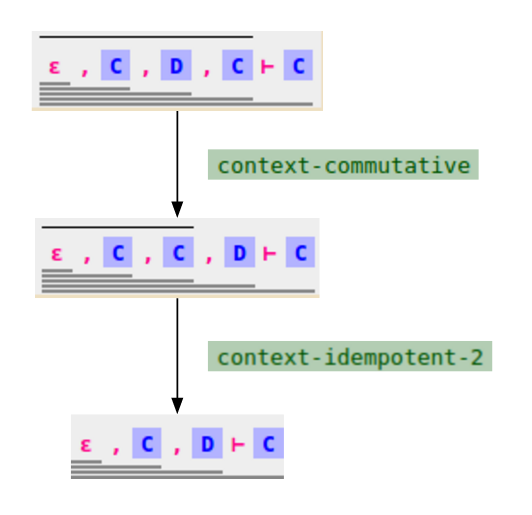
\includegraphics[width=\textwidth]{demo-meta-red}
\end{flushright}
\end{minipage}
\end{adjustwidth}
\end{frame}

\begin{frame}[fragile]
\frametitle{Implementation --- Elm language and its Signals}
\vspace{-1em}
\begin{center}
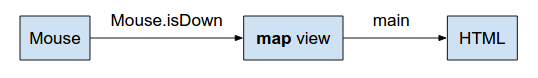
\includegraphics[width=0.9\linewidth,height=\textheight,keepaspectratio]{demo-imp-1}
\end{center}
\vspace{-1em}
\begin{adjustwidth}{2.5em}{0em}
\begin{lstlisting}[language=elm]
Mouse.isDown : Signal Bool

Signal.map  : (a -> b) -> Signal a -> Signal b

view : Bool -> Html
view is_clicked =
  if is_clicked then text "bar"
                else text "foo"

main : Signal Html
main = Signal.map view Mouse.isDown
\end{lstlisting}
\end{adjustwidth}
\end{frame}

\begin{frame}[fragile]
\frametitle{Implementation --- Model-Controller-View (MCV)}
\vspace{-1em}
\begin{center}
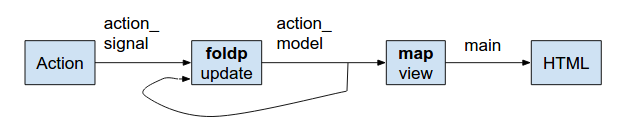
\includegraphics[width=0.9\linewidth,height=\textheight,keepaspectratio]{demo-imp-2}
\end{center}
\vspace{-1em}
\begin{adjustwidth}{2em}{0em}
\begin{lstlisting}[language=elm,basicstyle=\scriptsize\ttfamily,]
Signal.foldp : (a -> b -> b) -> b -> Signal a -> Signal b

update : Action -> Model -> Model
view   : Model -> Html

action_signal : Signal Action
action_signal = Signal.merge mailbox.signal keyboard_signal

model_signal : Signal Model
model_signal = Signal.foldp update init_model action_signal

main : Signal Html
main = Signal.map view model_signal
\end{lstlisting}
\end{adjustwidth}
\begin{flushright}
Remark: this is the \emph{simplified} version of Phometa main entry.
\end{flushright}
\end{frame}

\begin{frame}
\frametitle{Strengths, Limitation, and Future Work}

\begin{itemize}
\item Has extra features over the traditional derivation system such as prove by
  lemma, cascade premise, and meta-reduction.
\item Less learning curve than mainstream proof assistants.
\item The program always in consistent state\\i.e.\ impossible to create an
  invalid proof.\\[3em]
\item Phometa need to load the entire proof repository when start.
\item Theorem building process should be more automatic.
\item Nodes should be able to be exported into \LaTeX\ source code.
\item Modules should be able to import nodes from other modules.
\end{itemize}
\end{frame}

\begin{frame}
\frametitle{Achievement  \& Conclusion}

\begin{itemize}
\item Finished designing Phometa specification in such a way \\to keep it simple
  yet be able to produce a complex proof.\\ [1em]
\item Finished implementing Phometa, as you have seen in the demo.\\ [1em]
\item Encoded these formal systems in the standard library.
  \begin{itemize}
  \item Propositional Logic
  \item Simple Arithmetic
  \item Typed Lambda Calculus\\ [1em]
  \end{itemize}
\item Wrote a tutorial for newcomers to use Phometa\\(Chapters 3, 4, A, B, C in
  the report). \\[1em]
\item Phometa is ready to be used as a replacement\\of the traditional derivation system.
\end{itemize}
\end{frame}

\begin{frame}
\frametitle{Questions \& Answers}

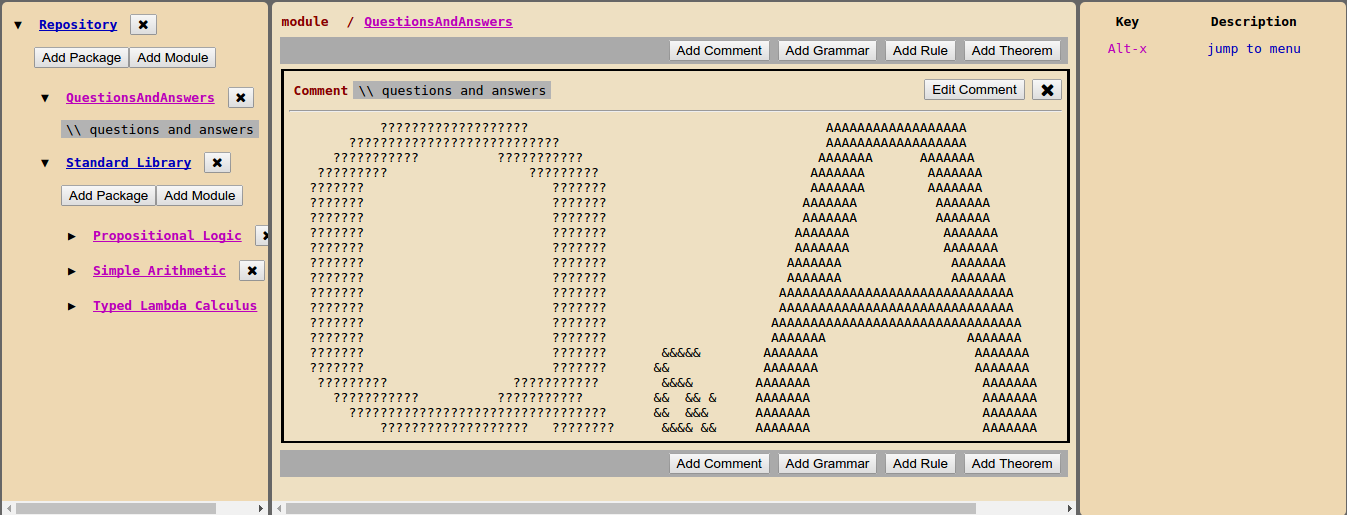
\includegraphics[width=\linewidth,height=\textheight,keepaspectratio]{demo-questions-and-answers}

\end{frame}


\begin{frame}
\frametitle{Thank You}

\begin{center}
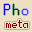
\includegraphics[width=0.5\linewidth,height=\textheight,keepaspectratio]{../logo}
\end{center}

\end{frame}

\end{document}
